\documentclass{book}

\usepackage{amsmath}
\usepackage{amsthm}
\usepackage{url}
\usepackage{xcolor,graphicx}
\usepackage{clrscode3e}
\usepackage{hyperref}
\usepackage{tikz}
\usepackage{csquotes}

\graphicspath{ {images/} }

\begin{document}

\part{Algorithms 1}

\section*{2.4.30 Dynamic-median finding.}
\begin{verbatim}
if key <= V
  if need to move a element from maxPQ to minPQ
    insert key to maxPQ with swim
    extract maxPQ.top to u
    insert u to minPQ with swim
    save maxPQ.top to v
    replace minPQ.top with v without sink
  else
    insert key to maxPQ with swim
    save maxPQ.top to v
    replace minPQ.top with v without sink
else
  this cas is symmetric
\end{verbatim}

\section*{2.4 Multiway heaps}



Swim: $\log_{d}N$. Sink: $(d-1)\log_{d}N$.

For $d=3$, swin: $\log_{3}N = \frac{1}{\log3}\log N$ and sink:
$2\log_{3}N=\frac{2}{\log3}\log N$.

For $d=8$, swin: $\log_{8}N = \frac{1}{3}\log N$ and sink: $7\log_{8}N=\frac{7}{3}\log N$

For $d=16$, swin: $\log_{16}N = \frac{1}{4}\log N$ and sink:
$15\log_{16}N=\frac{15}{4}\log N$

For $d=1024$, swin: $\log_{1024}N = \frac{1}{10}\log N$ and sink:
$1023\log_{1024}N=\frac{1023}{10}\log N$

\section*{3.2 Proposition C}

Equation 1 is based on Law of total expectation.

\begin{align*}
C_n &= \frac{C_0 + C_{N-1}+(N -1)}{N} + \frac{C_1+C_{N-2} + (N-1)}{N} + ... +
\frac{C_{N-1}+C_0+(N-1)}{N} (1)\\
C_n &= N - 1 + \frac{C_0 + C_{N-1})}{N} + \frac{C_1+C_{N-2})}{N} + ... + \frac{C_{N-1}+C_0}{N} \\
NC_N &= (N - 1)N + 2(C_0+C_1+...+C_{N-1}) \\
(N-1)C_{N-1} &= (N-2)(N-1) + 2(C_0+C_1+...+C_{N-2}) \\
NC_N &=2(N-1) + (N+1)C_{N-1} \\
\frac{C_N}{N+1} &= \frac{C_{N-1}}{N} + \frac{2(N-1)}{N(N+1)} \\
\frac{C_N}{N+1} &\le \frac{C_{N-1}}{N} + \frac{2}{N+1}
\end{align*}


\begin{align*}
\frac{C_N}{N+1} &\le \frac{C_{N-1}}{N} + \frac{2}{N+1} \\
\frac{C_{N-1}}{N} &\le \frac{C_{N-2}}{N-1} + \frac{2}{N}
\end{align*}

\begin{align*}
\frac{C_N}{N+1} &\le \frac{C_{N-2}}{N-1} + + \frac{2}{N} + \frac{2}{N+1} \\
\end{align*}

\part{Algorithms 2}
\section*{5.5 Proposition U}

The proposition says:

\textquote{Now consider an optimal trie $T$ for ($s_1$, $r_1$), ..., ($s_r$,
  $f_r$), of height $h$. Note that that ($s_i$, $f_i$) and ($s_j$, $f_j$) must be
  at depth $h$ (else we could make a trie with lower external path length by
swapping them with nodes at depth $h$).}

So there must at least two nodes at depth $h$. Let us prove that any internal
nodes in an optimal trie $T$ must have two children. Consider the following
trie $T$. Node $2$ is an internal node with only one child. An trie $T'$ can be obtained
by just replacing node $2$ with node $3$. $T'$ still corresponds to a prefix-free
code. And $W(T') < W(T)$ which contradicts the fact what $T$ is an optimal trie.

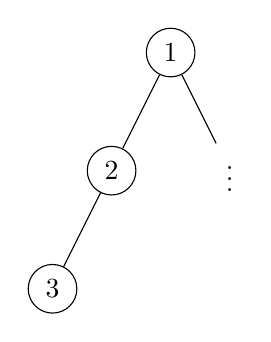
\begin{tikzpicture}
\node[circle,draw](z){$1$}
  child{
    node[circle,draw]{$2$} child{node[circle,draw] {$3$}} child[missing] }
    child{node {$\vdots$}};
\end{tikzpicture}

\section*{Time Complexity of Huffman Compression}

The time complexity if $N + R \lg R$. The time complexity of \verb+buildCode+
and \verb+writeTrie+ is $O(M)$ ($M$ is the number nodes in the Trie). Now let's
prove that $M \sim O(R)$.  It can be proved by induction that for a binary tree
with only degree-$2$ internal nodes, $\#nodes < 2 \cdot \#leaves$. So we can have $M <
2R$.

\part{Analysis of Algorithms}
\chapter{Chapter One Analysis of Algorithms}
\section*{Exercise 1.14}

It is obvious that $A_{0} = 0$, $A_{1} = 0$. Multiply the equation $N$ and $N-1$, we
have:

\begin{align*}
  NA_{N} &= N + 2 \sum_{i \leq j \leq N} A_{j-1} \\
  (N-1)A_{N-1} &= (N-1) + 2 \sum_{i \leq j \leq N-1} A_{j-1}
\end{align*}

Subtract the second equation from the first equation, we have:

\begin{align*}
NA_{N} - (N-1)A_{N-1} = 1 + 2 A_{N-1}
\end{align*}

Now rearrange terms to get a simple recurrence

\begin{align*}
  NA_{N} = 1 + (N+1)A_{N-1}
\end{align*}

This can be solved by dividing both sides by $N(N+1)$:

\begin{align*}
  \frac{A_{N}}{N+1} &= \frac{1}{N(N+1)} + \frac{A_{N-1}}{N} \\
  \frac{A_{N}}{N+1} &= (\frac{1}{N} - \frac{1}{N+1}) + \frac{A_{N-1}}{N}
\end{align*}

Iterating, we are left with the sum:

\begin{align*}
  \frac{A_{N}}{N+1} &= \frac{1}{2} - \frac{1}{N+1} \\
  A_{N} &= \frac{N-1}{2}
\end{align*}


\section*{Catalan Number}
$T_{0} = 1$

\begin{align*}
  T_{N} &= \sum_{0 \le k < N} T_{k}T_{N-1-k} + \delta_{N0} \\
\end{align*}

\begin{equation}
  T(z) \equiv \sum_{N \ge 0}T_{N}z^{N} = \sum_{N \ge 0}\sum_{0 \le k < N}
  T_{k}T_{N-1-k}z{N} + 1
\end{equation}

\begin{align*}
  T(z) &= 1 + \sum_{k \ge 0}\sum_{N > k}T_{k}T_{N-1-k}z^N \\
  T(z) &= 1 + \sum_{k \ge 0}\sum_{N > k}T_{k}T_{N}z^{N+K+1} \\
  T(z) &= 1 + z\bigg(\sum_{k \ge 0} T_k z^k\bigg)\bigg(\sum_{N \ge 0} T_N z^N \bigg) \\
  T(z) &= 1 + zT(z)^2 \\
  zT(z) & = \frac{1}{2}(1\pm\sqrt{1-4z})
\end{align*}

\section*{Exercise 1.15}

The following solution is based on \href{https://class.coursera.org/aofa-006/forum/thread?thread\_id=12}{Fortunato Flores's Solution}.

The exchanges in the first partition on the average can be computed as follows.

Say that the pivot has index $j$ after the partitioning is done. The number of
exchanges is the number of elements larger than the pivot which have index
smaller than j before the partitioning, alternatively the number of elements
smaller than the pivot which have index larger than j before the partitioning.


By our assumption (that the pivot has index $j$ after partitioning) we have $j$
elements smaller than the pivot and $N-1-j$ elements larger than the pivot.

There are two cases: one is when $j <= N-1-j$. Use $X$ to indicate the number of
larger elements before $j$. $X$ follows hypergeometric distribution. So $E[X] =
\frac{j(N-j-1)}{N-1}$. When $j > N-1-j$, by doing the same reasoning about the
number smaller elements after $j$, we can get the same result.

\begin{align*}
  B_{N} &= \frac{1}{N}\sum_{j=0}^{N-1}\frac{(N-1-j)j}{N-1} \\
  B_{N} &= \frac{1}{N(N-1)}\sum_{j=0}^{N-1}(N-1)j - j^2 \\
  B_{N} &= \frac{1}{N}\sum_{j=0}^{N-1}j - \frac{1}{N(N-1)}\sum_{j=0}^{N-1}j^2 \\
  B_{N} &= \frac{1}{N}\sum_{j=1}^{N-1}j - \frac{1}{N(N-1)}\sum_{j=1}^{N-1}j^2 \\
  B_{N} &= \frac{1}{N} \frac{(N-1)N}{2}- \frac{1}{N(N-1)}\frac{(N-1)N(2N-1)}{6} \\
  B_{N} &= \frac{N-1}{2} - \frac{(2N-1)}{6} \\
  B_{N} &= \frac{N-2}{6}\\
\end{align*}


\section*{Exercise 1.17, 1.18}


$$\frac{C_{N}}{N+1} = \frac{C_{M+1}}{M+2} + 2 \sum_{M+3 \le k \le N+1}\frac{1}{k}$$

\begin{align*}
  C_{M+1} &= (M+1) + 1 + \frac{1}{M+1} \sum_{1 \le j \le M+1} (C_{j-1} + C_{N-j}) \\
          &= M+2+\frac{2}{M+1}\sum_{1 \le j \le M+1} C_{j-1} \\
          &= M+2+\frac{2}{M+1}\sum_{0 \le j \le M} C_{j} \\
          &= M+2+\frac{2}{M+1}\sum_{0 \le j \le M} \frac{j(j-1)}{4} \\
          &= M+2+\frac{1}{2(M+1)}\Big(\sum_{0 \le j \le M} j^2 - \sum_{0 \le j \le M} j\Big) \\
          &= M+2+\frac{1}{2(M+1)} \frac{(M-1)M(M+1)}{3} \\
          &= M+2+\frac{(M-1)M}{6} \\
\end{align*}


$$\frac{C_{N}}{N+1} = 1 + \frac{{(M-1)M}}{6(M+2)} +  2 \sum_{M+3 \ge k \ge N+1}\frac{1}{k}$$

$$\frac{C_{N}}{N}= 1 + \frac{M}{6} + 2 (H_{N+1} - H_{M+2})$$

\begin{align*}
  C_{N} &= N + \frac{NM}{6} + 2N(\ln{N} - \ln{M}) \\
   &= 2N\ln{N} + \Big( 1 + \frac{M}{6} - 2\ln{M}\Big)N
\end{align*}

$$ f(M) = 1 + \frac{M}{6} - 2\ln{M}$$

$$ f'(M) = \frac{1}{6} - \frac{2}{M}$$
$$ f''(M) = \frac{2}{M^2}$$

$M = 12$

\end{document}

